\newpage
\fancyhead[R]{\sffamily\small\color{Muted}Vulkan / 镜面反射}
\section{镜头外的倒影}
镜子工作室的灯牌挂在相机后方。只查屏幕深度的 SSR 能看见墙和镜框，却找不到灯牌。打开「屏幕外反射」后，SSR 会先在屏幕上找。找不到时，显卡再沿反射方向查场景里的三角形，算出最近的表面朝镜子送来多少光。

\begin{figure}[H]\centering
\begin{minipage}{.45\linewidth}\centering\small\sffamily 只查屏幕\par\smallskip
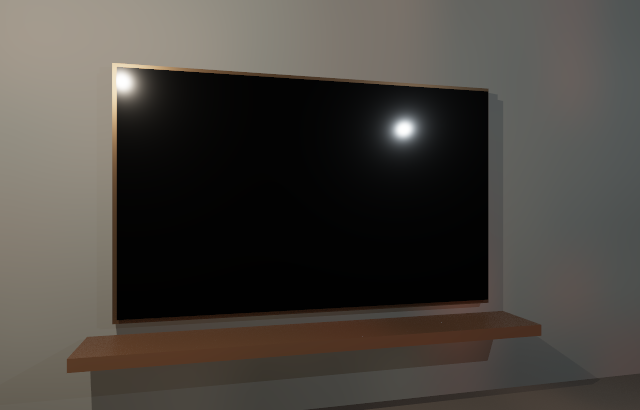
\includegraphics[width=\linewidth]{scene-reflections/mirror-screen.png}\par\vspace{3pt}
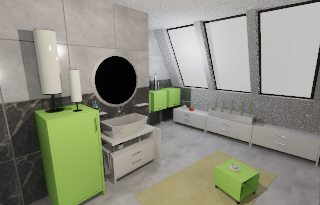
\includegraphics[width=\linewidth]{scene-reflections/bathroom-screen.png}
\end{minipage}\hfill
\begin{minipage}{.45\linewidth}\centering\small\sffamily 屏幕上找不到时再查场景\par\smallskip
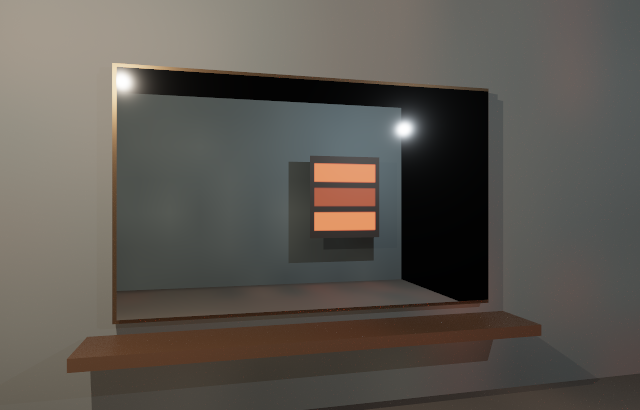
\includegraphics[width=\linewidth]{scene-reflections/mirror-scene.png}\par\vspace{3pt}
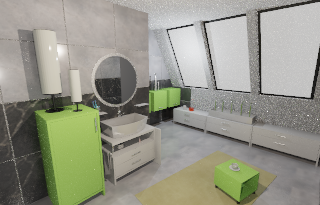
\includegraphics[width=\linewidth]{scene-reflections/bathroom-scene.png}
\end{minipage}
\caption{第 24 帧的场景面板，从 RenderDoc 回放导出。上排可以直接辨认镜中的横条灯牌。下排是 NVIDIA RTXGI 浴室，注意洗手盆上方的圆镜，右图里能看见对面墙上的明暗分界。}
\end{figure}

{\smalltable\noindent\begin{tabularx}{\linewidth}{@{}Xlrrr@{}}\toprule
场景和画幅 & 反射查找方式 & 事件编号 & 找到物体的像素 & GPU 毫秒\\\midrule
\mirrorTimingRows
\bottomrule\end{tabularx}\par}

两组都开启 SSR。找到物体的像素会在输出的第四个分量写入 1，照见黑框也算一次。用 RTX 5070 Ti Laptop GPU 运行 Debug x64 编辑器，在 RenderDoc 1.47 中预热一次，再回放 11 次。表中是单条反射计算命令的 GPU 耗时中位数。

浴室的画幅小，打开屏幕外反射后的用时却更长。除了统计像素，还值得数一数每条光线检查了多少三角形。下一步可以把屏幕上没找到物体的像素集中起来，再查场景。整理和追踪的时间都要计入，才能判断这样做能否更快。

{\small\color{Muted}逐次计时、原帧校验值和场景设置见 \path{output/profiling/scene-reflections/frames.json}。\par}
